\documentclass{standalone}
\usepackage{pgfplots}
\usepackage{amsmath}
\usepgfplotslibrary{colormaps}

\pgfplotsset{compat=newest}

%%%% Differential system %%%%%
%\def\c{1}
\def\xdot{x*(1-x-y)}
\def\ydot{y*(1-x-y)}
%%%%%%%%%%%%%%%%%%%%%%%%%%%%%%

\begin{document}
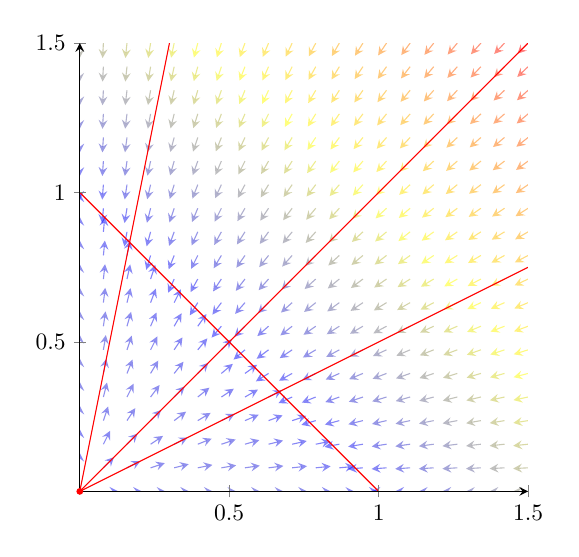
\begin{tikzpicture}[every node/.style={scale=0.85}]
  \begin{axis}[
      axis lines=middle,
      xmin=0,xmax=1.5,
      ymin=0, ymax=1.5,
      zmin = 0, zmax = 1, % to prevent a warning
      view={0}{90},
      % xlabel = {$x$},
      % ylabel = {$y$},
      axis equal image,
      trig format plots=rad,
      %colormap/vidris,
    ]
    \def\xmax{\pgfkeysvalueof{/pgfplots/xmax}}
    \def\xmin{\pgfkeysvalueof{/pgfplots/xmin}}
    \def\ymax{\pgfkeysvalueof{/pgfplots/ymax}}
    \def\ymin{\pgfkeysvalueof{/pgfplots/ymin}}
    \addplot3[
    opacity = 0.5,
    point meta={sqrt((\xdot)^2+(\ydot)^2)},
    samples=20,
    domain=\xmin:\xmax,
    y domain=\xmin:\xmax,
    quiver={
    u={\xdot/sqrt((\xdot)^2+(\ydot)^2)},
    v={\ydot/sqrt((\xdot)^2+(\ydot)^2)},
    colored = {mapped color},
    scale arrows=0.05,
    every arrow/.append style={-{stealth}}
    }
    ] {0};
    \foreach \i in{1-x,x,5*x,x/2}{
        \addplot[
          samples=200,
          % samples y=100,
          domain=\xmin:\xmax,
          %y domain=\xmin:\xmax,
          red
        ] {\i};
      }
    \addplot[thin,mark=*,only marks, mark size=1pt,red] coordinates {
        (0,0)
      };
  \end{axis}
\end{tikzpicture}
\end{document}